\chapter{Theoretische Grundlagen}
Der Bicycle Computer basiert auf Energy Harvesting. Was Energie ernten bedeutet und welche Art von Energy Harvesting in dieser Arbeit benutzt wird, wird im ersten Unterkapitel \ref{t_harvesting} beschrieben. \\
Da die gewonnene Energie im $\mu$W-Bereich liegt, ist ein Sammeln der Energie notwendig, sodass Leistungen im mW-Bereich zur Verfügung stehen. Ansätze zur Umsetzung zum Sammeln und Weiterleiten von Energie werden im Unterkapitel \ref{t_energy_management} beschrieben.\\ 
Die gewonnene Energie darf nicht sofort verbraucht werden, deshalb ist auch ein Power Mangement notwendig. Dieses regelt, wie schnell wie viel Energie verbraucht werden kann (siehe \ref{t_power_management}).\\
Als letzte Stufe in der Umsetzung ist eine energiearme Kommunikation notwendig. Da bietet die Bluetooth Low Energie Technologie ideale Voraussetzungen. Das Protokoll und die Technologie werden im letzten Grundlageteil \ref{t_ble} vorgestellt.


% 2.1-------------------------------------------------------------------
\section{Energy Harvesting}\label{t_harvesting} 

\glqq Mit Energy Harvesting ... wird die Gewinnung von elektrischer Energie in kleinen Mengen aus dem Umfeld elektronischer Geräte für deren Betrieb bezeichnet.\grqq \cite{harvesting}. \\

Als erstes werden Methoden zur Energiegewinnung vorgestellt \ref{harv_arten} und danch die im Bicycle Computer verwendete Harvesting Art genauer beschrieben \ref{harv_bewegung}. Als letztes wird der Unterschied zwischen den Harvestingmethoden festgehalten. Denn diese Unterschiede werden in der Implementation des Bicycle Computers wichtig


\subsection{Energy Harvesting Methoden}\label{harv_arten} 

Bekannte Methoden sind die Solarzelle, die aus der Energie der Sonnenstrahlen Strom erzeugt, die Thermogeneratoren (TEG), die aus Umgebungswärme Energie gewinnen,  passive RFID-Tags, die aus der elektromagnetischen Strahlung Energie gewinnen und der piezoelektrische Effekt, der mechanischen Druck in elektrische Spannung umwandelt.\\


Da der im Prototyp verwendete Energy Mangement-Chip \ref{t_em8500} für die Energieoptimierung von Solarzellen oder von Thermogenaratoren spezialisiert ist, werden diese zwei Methoden vorgestellt. 

\subsubsection{Energy Harvesting mit einer Solarzelle}\label{harv_solarzelle} 


Bei der Umwandlung von Elektromagnetischen Wellen (Licht) in Strom wird eine spezielle Eigenschaft des Siliziums genutzt: Führt man Silizium Energie zu, entstehen freie Ladungsträger, bzw. Elektronen und Löcher. "Um aus diesen Ladungen einen elektrischen Strom zu erzeugen, ist es nötig, die erzeugten freien Ladungsträger in unterschiedliche Richtungen zu lenken; dies geschieht ... durch ein internes elektrisches Feld, welches durch einen p-n-Übergang erzeugt werden kann." (https://de.wikipedia.org/wiki/Solarzelle ((21.5.16:12:04), 12:22)
Auf der einen Seite sammelt sich positive, auf der anderen Seite negative Ladung an. Werden diese verbunden, entsteht ein Strom. \\

(http://sms.ckw.ch/content/ckwsms/de/startseite/mittelstufe/solaranlage-erklaert.html   (21.5.16:12:04))Abschnitt Funktionsprinzip). \\

Diese Harvestingmethode produziert ein Gleichstrom. Die Spannung am Ausgang ist konstant, da es sich um eine Stromquelle handelt (stimmt das ?). Grössen- und materialabhängig kann Energie im kW-Bereich gesammelt werden.



\subsubsection{Energy Harvesting mit einem TEG}\label{harv_TEG} 
TEG steht für Thermoelectric Generator und bezeichnet eine Konstruktion, die aus einem Temperaturunterschied elektrische Spannung erzeugt. (https://de.wikipedia.org/wiki/Thermoelement)\\
Erzeugt wird die Spannung am Ende zweier metallischer Leiter aus unterschiedlichem Material, die an einem Ende verbunden sind.(https://de.wikipedia.org/wiki/Thermoelement)\\


Diese Harvestingmethode produziert eine Gleichspannung. Die produzierte Spannung ist vergleichsweise klein und bewegt sich im Bereich einiger 10 $\mu$ V pro $1^\circ C$ Temperaturdifferenz.


\subsection{Energy Harvesting über Bewegungsindktion}\label{harv_bewegung} 
Beim Bicycle Computer wird Energie über Bewegungsinduktion gewonnen. Die Funktionsweise ist in der Machbarkeitsstudie beschrieben \cite{PA_bicycle} S.8. : 

Befindet sich eine Spule in einem \textit{dynamischen} \glqq Magnetfeld\grqq, wird in der Spule eine Spannung induziert. Dies sieht man in der Formel (\ref{Formel_induzSpannung}).

\begin{equation}
    U_{ind}=-\frac{d}{dt}\intop A\,dB \ \label{Formel_induzSpannung} 
\end{equation}

Der magnetische Fluss $B$ durch die Fläche einer Spule $A$ ist gleich dem magnetischen Fluss $\phi$. Hat die Spule mehrere Wicklungen $N$, so verstärkt sich der magnetische Fluss proportional. 

 
\begin{equation}
    \frac{d}{dt} \int A\,dB=\phi\cdot N\
\end{equation}

Verläuft der \textbf{magnetische Flus???}s $\phi$ senkrecht zur Fläche der Spule $A$ kann das Integral durch eine Multiplikation ersetzt werden (siehe Formel\label{Formel_senkrecht}). 
 
\begin{equation}
    \frac{d}{dt} \int A\,\perp\, dB=\frac{d}{dt}\int \phi\cdot N=B\cdot A\cdot N\ \label{Formel_senkrecht} 
\end{equation} 
  
 
In diesem Fall berechnet sich die induzierte Spannung in einer Spule vereinfacht mit
\begin{equation}
    U_{ind}= - N \cdot A \cdot B
\end{equation}

Das dynamische Magnetfeld wird durch das Bewegen, oder im Fall eines Fahrrads einem Vorbeiziehen, eines Magneten an einer fix verankerten Spule erzeugt.
Die produzierte Spannung hängt von drei Kriterien ab:

Eine induzierte Spannung wird somit durch folgende vier Faktoren beinflusst:
\begin{enumerate}
    \item die eingeschlossene Fläche $A$ der Spule    
    \item die magnetische Flussdichte des Magneten $B$ 
    \item die Anzahl Windungen $N$ der Spule und
    \item die Bewegungsgeschwindigkeit $v$ des Magneten, welche Einfluss auf $dt$ hat
\end{enumerate}

Diese Harvestingmethode produziert einen Wechselstrom. Ein Gleichrichter und einen Kondensator zur Glättung der Rippelspannung ist nach der Energiegewinnung notwendig. Die Leistung der produzierten Spannung geht vom $\mu$W-Bereich bis zu für die Industrie optimierten Anlagen mit Leistung MW-Bereich wie z. B. durch Drehstrom-Generatoren.\\



\subsection{Unterschiede der Methoden}\label{harv_diff} 

Der grösste Unterschied besteht in der Art in der die Energie zur Verfügung steht. 

\subsubsection{Gleichmässige Energie versus gepulster Energie}
Die Solarzelle und ein TEG liefern Gleichstrom bzw. -spannung. Wodurch kein Gleichrichterschaltung und Glättung notwendig sind.\\

Die durch Bewegungsinduktion gewonnene Energie ist eine Wechselspannung. Im Fall des Bicycle Computers ist diese gleichzeitig gepulst. Die Energie ist somit nicht konstant da, sondern nur in Zeitintervallen.\\

\subsubsection{Konstanter Maximum Power Point zu dynamischem}
Die drei Harvester unterscheiden sich in ihrer Leistungskurve. Das Leistungsmaximum, der Maximum Power Point (MPP), liegt auf der Skala von Kurzschluss bis Leerlauf proportional an unterschiedlichen Stellen.  Bei einem TEG liegt das MPP in der Mitte dieser Skala. Die MPPT-Ratio beträgt 50 \%. Bei der Solarzelle liegt das Leistungsmaximum auf der Skala bei ca. 80 \% der maximalen Spannung. Die MPPT-Ratio ist 80 \%.  Bei der Bewegungsinduktion existiert kein fixe MPPT-Ratio. Wie bei der Spule, wandert das Leistungsmaximum aufgrund mehrerer Indikatoren (wie Geschwindigkeit des Magneten durch die Spule, Abstand von Magnet und Spule) auf der Skala hin und her.\\

Zur Verdeutlichung der Unterschiede sind für jedes Leistungsverhalten eine Graphik angefügt.\\

Das TEG hat unabhängig von der gewonnenen Energie und der Temperatur das Leistungsmaximum immer bei 50 \%. Die Graphik \ref{MPP_TEG} zeigt, dieses unabhängige Verhalten. 

\begin{figure}
 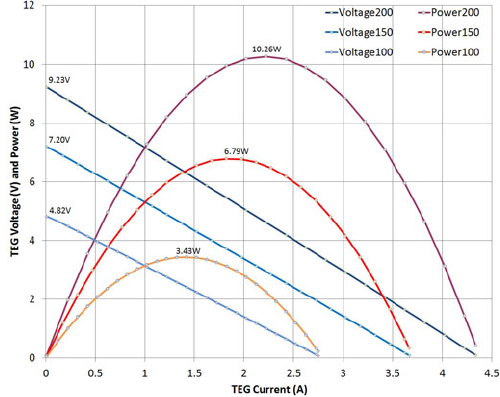
\includegraphics{2TheoretischeGrundlagen/imag/MPPTEG.png}\label{MPP_TEG} 
\caption{MPP TEG (\cite{MPP_TEG})}
\end{figure}


Graphik \ref{mpp_solar} zeigt, dass das Leistungsmaximum bei der Solarzelle unabhängig von der zur Verfügung stehenden Energie immer bei 80 \% liegt.

\begin{figure}
   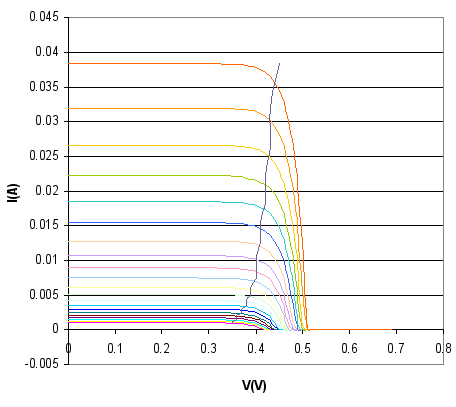
\includegraphics{2TheoretischeGrundlagen/imag/MPPSolar.png}\label{mpp_solar} 
   \caption{MPP Solarzelle }
\end{figure}

% \cite{mpp_solar}

Die Stelle des Leistungsmaximums wandert bei einer Spule und somit bei der Bewegungsinduktion auf der Skala. \\
Exemplarisch sind drei MPPT-Ratios einer Spule in der Graphik \ref{mpp_spule} abgebildet. In dieser Graphik zeigt sich der Einfluss des Abstands der Spule vom Magnetfeld auf die Stelle der maximalen Leistung. Diese Graphik wurde ausgewählt, weil beim Ausmessen des Harvesters der Abstand des Magneten als einer der Einflüsse festgestellt wurde.\\

Als interessanter für die Anwendung wurde der Einfluss der Geschwindigkeit, mit der der Magnet an der Spule vorbeizieht, genauer dokumentiert. Denn dieser Faktor ist durch den Nutzer direkt beeinflussbar (Graphik \ref{mpp_harvester}). \\


Über alle Messungen hinweg lässt sich grob über die MPPT-Ratio des Bicycle Computers sagen, dass sie sich zwischen 40 - 80 \% bewegt.

\begin{figure}
   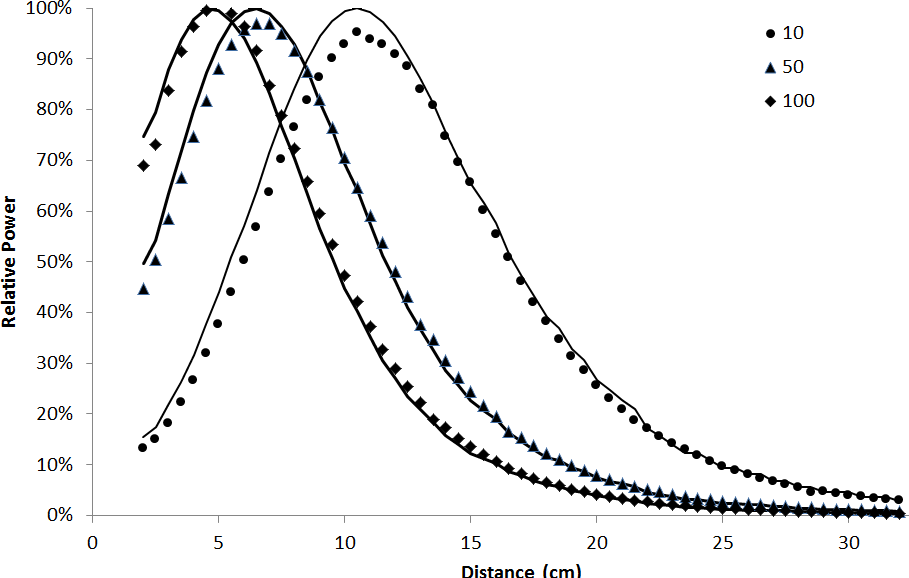
\includegraphics{2TheoretischeGrundlagen/imag/MPPSpule.png}
   \caption{MPP Spule}\label{mpp_spule} 
\end{figure}

%\cite{MPP_Spule}

\begin{figure}
   
\includegraphics{Idle.jpg}
   \caption{MPP Spule}\label{mpp_harvester} 
\end{figure}

\cite{MPP_Harv}


% 2.2-------------------------------------------------------------------
\section{Energy Management}\label{t_energy_management} 
Was wir machen: HRV Energie nicht direkt in sensortag, sondern in LTS speichern.

In der Bachelorarbeit ist bei der Umsetzung des Enerergymanagements der Chip EM8500 vorgegeben. Dieser IC ist von EM Microelectronics aus Marin (NE) entwickelt. %( Alternative Powermanagementsysteme sind z. B. : Booster TI, Analog Devices, E-Beas.)


Energy Management bezeichnet das Regeln von Energiezuständen, damit ein Optimum an Leistung aus einer Quelle bezogen werden kann.


%The EM8500 is an autonomous power management system able to manage power domains, power sources and storage elements \cite{datasheet_EM85}, p. 11.

Zu diesem Chip ist das Evaluation-Board EMEVB8500 (im Text mit EVB abgekürzt) entwickelt, welches das Aufsetzen eines energieoptimierten Systems unterstützt. 


\subsection{Regelung des optimalen Leistungsbezugs}

Generell MPP beschreiben, nicht EM MPP
Widerstandskurve als Graphik nehmen
MPP ist wie Leistungsanpasung

Wichtigster Punkt in der Energieoptimierung ist das Maximum aus der produzierten Energie herauszuholen. Die maximale Leistung ergibt sich beim MaximumPowerPoints (MPP), dem Punkte, an denen am effizientesten Leistung bezogen werden kann. 
Das EVB versucht die Quelle stets in der Nähe dieses Optimums zu betreiben. Dies geschieht über eine Innenwiderstand-Regelung, sodass die Eingangsleistung möglichst dem MPP entspricht.

Zweite Aufgabe beim Energiemanagement ist eine konstante Eingangsspannungen zu erzwingen. Das System kontrolliert periodisch den aktuellen (unregulierten) Spannungswert der Harvestingquelle. Hat sich der Wert mehr als 37 mV gegenüber der zur Zeit aktuellen Regelspannung geändert, wird der neue Wert als Spannungsreferenz zum Regeln genommen. Die Abbildung \ref{RegelungSpannung} zeigt das Anpassen der Spannungslevel alle s. Die periodischen Kontrollmessungen alle 8 s verursachen kurze Spannungsspitzen. Diese entstehen bei der Kurzschlussmessung, für den akutellen Stromwert.


\begin{figure}    
    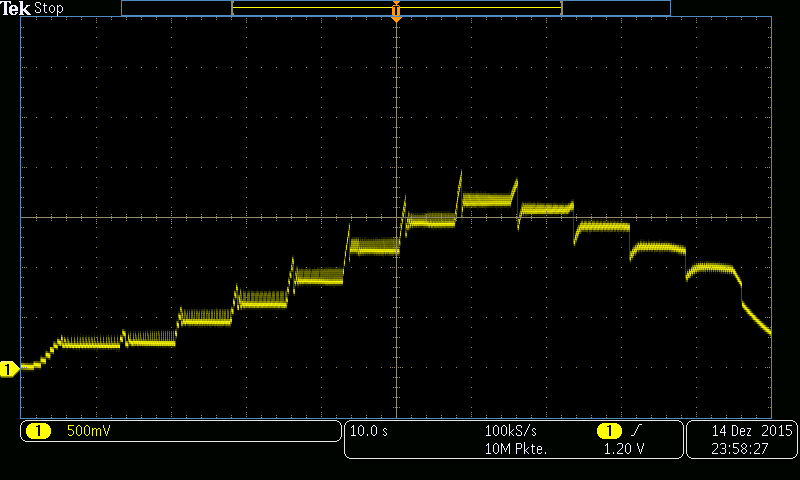
\includegraphics{2TheoretischeGrundlagen/imag/RegelungVHRV.png}
    \caption{Spannungswerte Modell der Machbarkeitsstudie}\label{RegelungSpannung} 
\end{figure}

Entsprechen die Konfigurationen auf dem EVB nicht dem Verhalten der Eingangsquelle, so entstehen keine konstanten Spannungswerte an der Harvestingquelle, was Abbildung \ref{falscheRegelung} zeigt.

\begin{figure}
    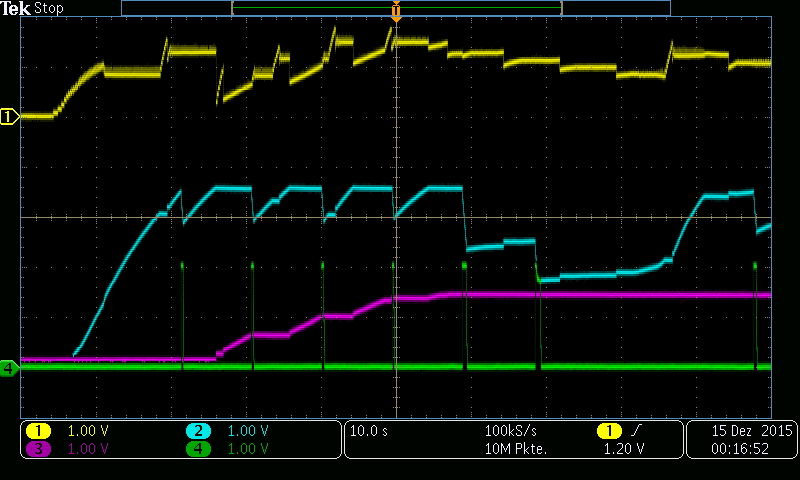
\includegraphics{2TheoretischeGrundlagen/imag/falscheRegelung.png}
    \caption{Spannungswerte Modell der Machbarkeitsstudie}\label{falscheRegelung} 
\end{figure}

Dritter Punkt ist der Aufbau von Energiespeichern. Diese sollen so viel Energie speichern, wie eine gewisse Aktion braucht. Das Energiemanagmenet kennt für jede Aktion den Energieverbrauch und löst, bei genügend Speicherenergie eine Aktion laufen (siehe Berechnung der Kondensatoren).

Das Berechnen der Schwellwerte und der Kondensatoren detaillierter in Kapitel XXXXS.






\subsubsection{Energie Management Chip EM8500}\label{t_em8500} 

MPP:
- start bei 50 \% (wir bei 40), und grobe Schritte (unten . direkt auf 60 \%, dann 67 \%). 

%Sobald genügend Startenergie bereit steht, wacht der EM8500-Chips auf. Neben dem Setzen der Konfigurationen aus dem EPROM kontrolliert der Chip als erstes den aktuellen Speicherzustand der angeschlossenen Speicher.

%Die Engeriequelle wie auch die angeschlossenen Speicher haben eigene Pins, die ihren Zustand übermitteln\cite{datasheet_EM85}, p.11. 



% 2.3-------------------------------------------------------
\section{Power Management}\label{t_power_management} 
- Zeichnen des Init, sleep, Aufwachen

Zur Verwaltung der gegebenen Energie ist der Microcontroller gegeben. Es handelt sich um einen Cortex M3, der sich auf dem Sensortag von Texas Instruments befindet. Die zentralen Eigenschaften dieses Boards und die Funktionsblöcke befindet sich im Anhang \ref{anhang_sensortag}.

\subsection{Fähigkeiten eines Low Power Microcontrollers}
  
Low Power Microcontroller können Gebiete des Prozessors oder von Periopherieelementen temporär ausschalten. Das System befindet sich im Standby Modus. Nur die für die Applikation unabdingbaren Aktivitäten laufen mit niederstem Takt weiter. Über Interrupts können einzelne Bereich aufgeweckt werden, die ihre Aktionen ausführen und danach geht das System wieder in den Standby Modus.

Bild: Energie-Langzeitmessung BLE versenden
Beschriften mit aktiv und standby modus

Zu den unabdingbaren Aktivitäten eines laufenden Microcontrollers gehört das Refreshen (Neuladen) der Register mit den Systemeinstellungen. Diese Refreshing-Peaks sieht man im Standby Modus.



\section{Aufsetzen des Low Power Microcontrollers}
%Üblicherweise wird das RTOS-Betriebssystem von TI für Low Power Applikationen benutzt. 
(Die Low-Power Programmbeispiele von TI basieren auf RTOS, ebenso die Dokumentation zu Low Power Applikationen, was zu viel Energie verbraucht (korrekt, wie belegen?). )

Konfiguration der CPU (system.h, config.h)
Einstellungen Active Mode: Sensoren, Wireless Processor, SPI-Kommunikation

Einstellungen sleep Mode: Abstellen

PowerDomain ausschalten
Clk

GPiO Konfigurieren (gpio.h, board.h)
Event anstelle von Interrupt
Synchronisation
timer, oder systick oder GPiO signal. Wake up

Aktivitäten aufsetzen






% 2.4-------------------------------------------------------------------
\section{Bluetooth Low Energy}\label{t_ble} 

Unterschied zu Bluetooth

Spezifikationen





